\begin{frame}
\section{}
Consider the following code snippet for convolution

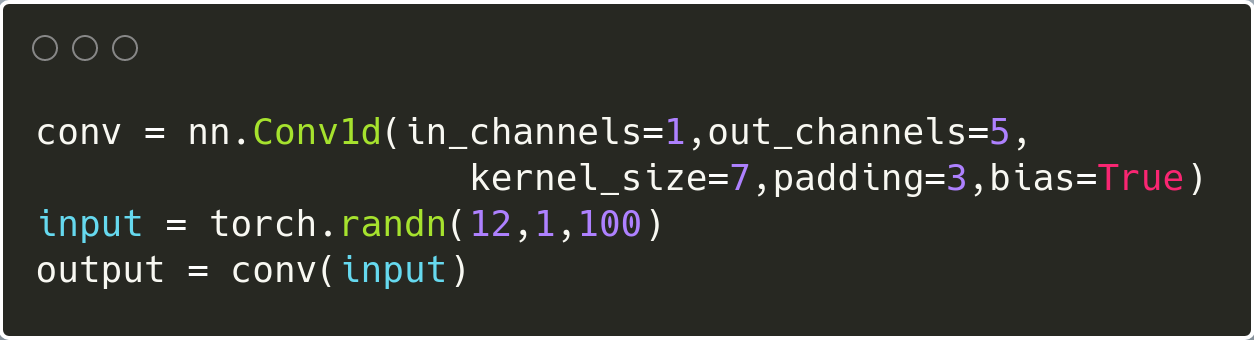
\includegraphics[width=0.7\textwidth]{images/quiz_4_4_5_1.png}

What is the shape of output?
% FIB

\end{frame}


\begin{frame}
\section{}
Consider the following code snippet for convolution

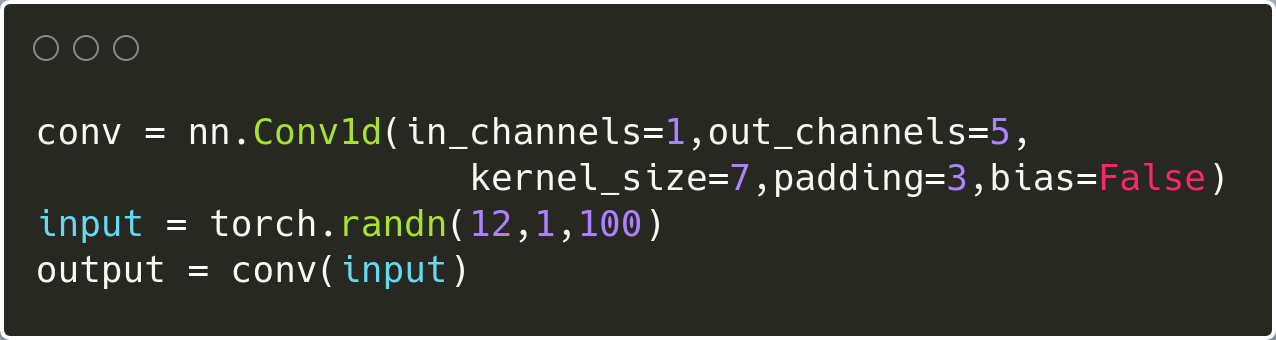
\includegraphics[width=0.7\textwidth]{images/quiz_4_4_5_2.png}

What is the shape of output?
% FIB

\end{frame}


\begin{frame}
\section{}
Consider the following code snippet for convolution

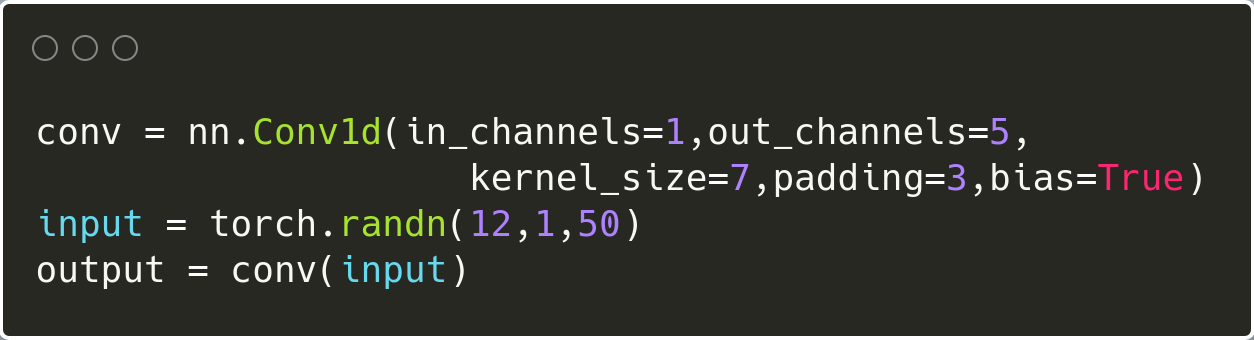
\includegraphics[width=0.7\textwidth]{images/quiz_4_4_5_3.png}

What is the shape of output?
% FIB

\end{frame}


\begin{frame}
\section{}
Consider the following code snippet for convolution

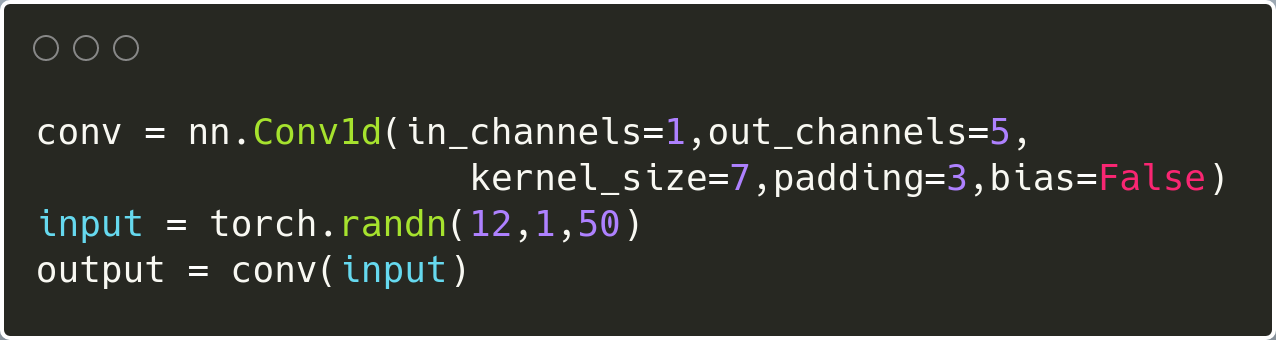
\includegraphics[width=0.7\textwidth]{images/quiz_4_4_5_4.png}

What is the shape of output?
% FIB

\end{frame}


\begin{frame}
\section{}
Consider the following code snippet for convolution

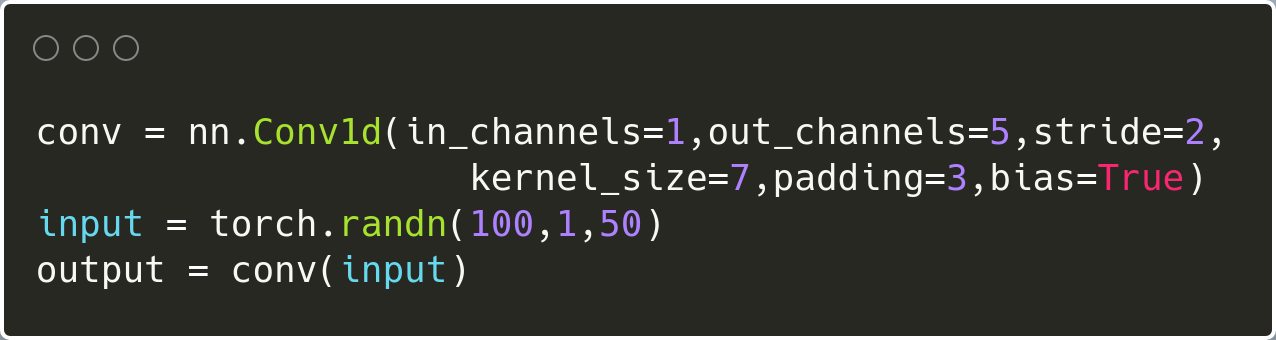
\includegraphics[width=0.7\textwidth]{images/quiz_4_4_5_5.png}

What is the shape of output?
% FIB

\end{frame}


\begin{frame}
\section{}
Consider the following code snippet for convolution

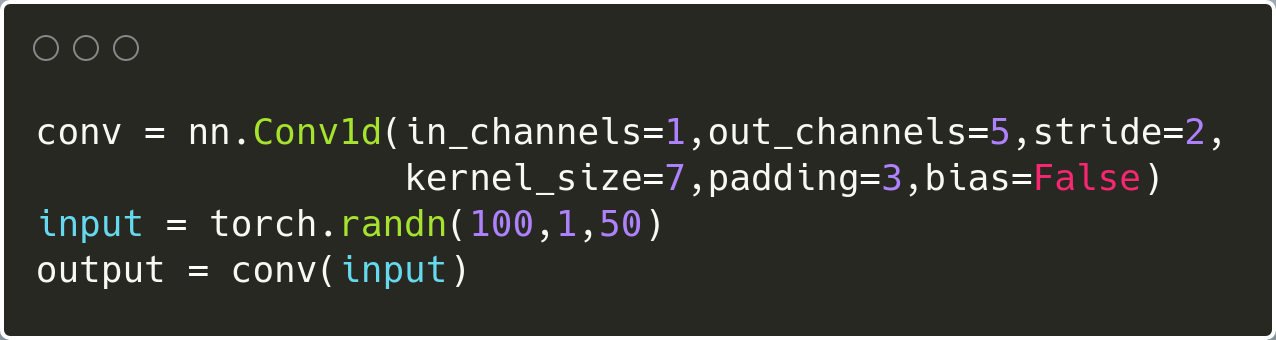
\includegraphics[width=0.7\textwidth]{images/quiz_4_4_5_6.png}

What is the shape of output?
% FIB

\end{frame}
